\section{論文の選択理由}

本節では今回のレポート課題においてなぜこの論文を選択したかについて,
画像マッチングの他の画像認識タスクへの応用性,およびロボットなどによる実環境タスク
への応用性の二つの観点から述べる.

まず画像認識タスクとして応用可能なものとして以下の様なものが考えられ,
以下ではそのそれぞれに関して画像マッチングの有効性を具体的に述べる.

\begin{description}
  \item[物体識別]\mbox{}\\
    画像内の物体にラベルを予測するタスク.
  \item[物体検出及びセグメンテーション]\mbox{}\\
    画像内の物体の位置とラベルを予測するタスク.
  \item[物体トラッキング]\mbox{}\\
    複数の画像にまたがって物体IDを保ったままその位置を予測するタスク.
  \item[三次元復元]\mbox{}\\
    二次元画像から姿勢とメッシュモデルなどの三次元的な情報に変換するタスク.
\end{description}

``物体識別''では既に意味の与えられている画像と新しい画像とを比較して,
その一致度合いによって新しい画像に対して意味を与えることができる.
例えば
\figref{matching_for_classification_cola}
% \footnote{http://www.umiacs.umd.edu/research/SRVC/architecture.htm}
においてSIFTによる画像マッチングの例を示すように,
コーラが映っているとわかっている画像とコーラが映っているがその情報が与えられていない画像
が与えられたときに,画像のピクセルごとの一致度を正しく予測できれば,
新しい画像において一致する部分は多いはずであり,それによって新しい画像にも
コーラが映っているというラベルを付けることができる.

\begin{figure}[htbp]
  \centering
  \begin{tabular}{c}
  \subfloat[]{
    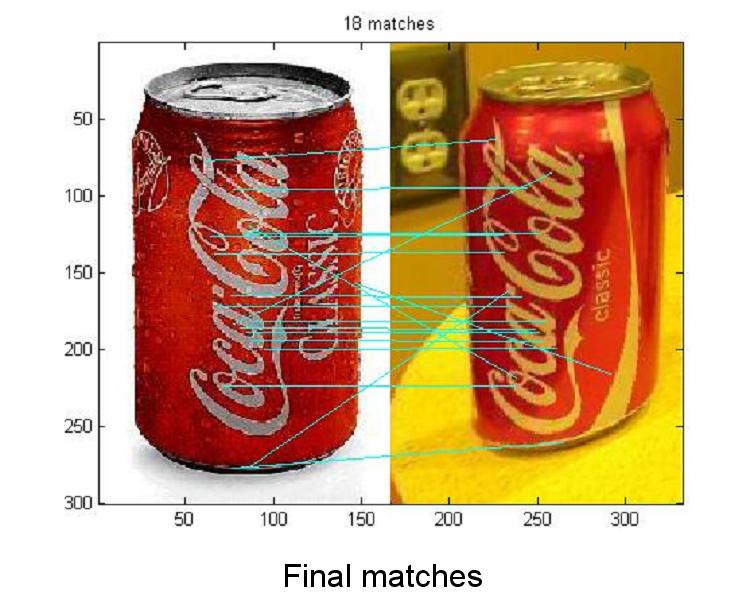
\includegraphics[width=0.44\columnwidth]{figs/matching_for_classification_cola}
    \label{figure:matching_for_classification_cola}} \\
  \end{tabular}
  \begin{tabular}{c}
  \subfloat[]{
    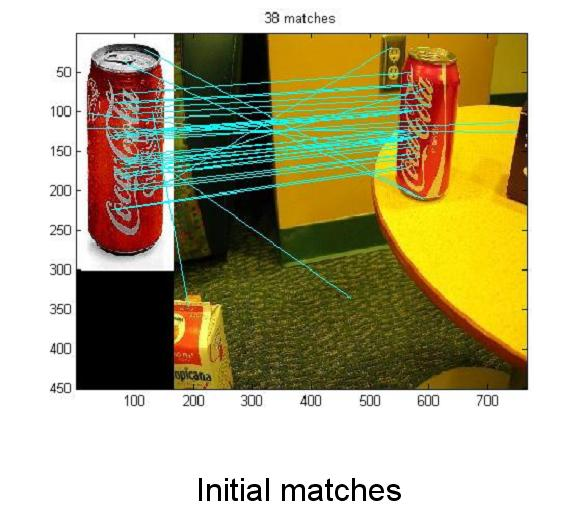
\includegraphics[width=0.38\columnwidth]{figs/matching_for_segmentation_cola}
    \label{figure:matching_for_segmentation}}
  \end{tabular}
  \caption{Examples of correspondence recognition applications \protect\footnotemark}
\end{figure}
\footnotetext{http://www.umiacs.umd.edu/research/SRVC/architecture.htm}

``物体検出及びセグメンテーション''は物体識別とともに位置の同定タスクが組み合わさったもの
と考えることができるが,物体のラベルの他に位置の情報も画像とともに与えられているとすれば,
\figref{matching_for_segmentation}
%\footnote{http://www.umiacs.umd.edu/research/SRVC/architecture.htm}
においてSIFTによる画像マッチングの例を示すように新しい画像でも
ピクセルごとのマッチングを行うことによってその領域にどのラベル
の物体があるかということがわかり,物体検出の結果とすることができる.
通常の物体検出\cite{girshick14CVPR}では画像の各注視領域(ROI)において
何の物体であるかということを識別しピクセルごとの密な認識結果を得ることはできないため,
画像マッチングは密な位置同定が可能という点で有効であると言える.
一方で物体セグメンテーションと比較すると,
通常の物体セグメンテーション\cite{long_shelhamer_fcn}
はピクセルごとの各物体クラスを予測するもので,
どこまでが一つの物体であるかを予測することはしないため,
例えば人が二人いる画像において``人''というクラスがある領域はわかるが
人が隣接している場合には数まではわからない.
それに対して画像マッチングを用いた物体セグメンテーションではピクセルごと
の一致性がわかっているため,元画像で一人であった部分を切り出すことが可能であり,
クラスのみを推定する物体セグメンテーションに特化したものと比べ
各物体を切り出すことができるという点で有効であると言える.

``物体トラッキング''では物体検出とセグメンテーションとの比較の際に述べたように,
画像マッチングを応用した場合には2フレーム間において同一性を担保したまま
密なセグメンテーションを行う事ができる.
そのため,トラッキングにおいて必要となる同一性とROI以上の位置正確性を持ったセグメンテーション
という二つの必要要件を満たすことができる.

``三次元復元''では通常,二次元画像に対して三次元モデルとのマッチングを行い,
モデルの姿勢を推定することによって,二次元では見えていない部分の三次元形状を得る.
画像マッチングにおいては,全く同じ物体でない場合でもクラスが同じであればマッチングを行う
ことができるため,それによって物体の対応点によって既知モデルを変形し,新しい物体に
適した三次元モデルとしてフィッティングを行うことが可能であると考えられる.
これにより,通常の三次元モデルフィッティングにおいて問題となる新物体への適応性
を実現する可能性があると言える.

上に述べたように画像マッチングタスクにおける認識器は他のさまざまなタスクへの応用が可能であると
期待される.
もちろん,それぞれのタスクに特化した研究というのはなされているが
% classification
\cite{vgg}
% detection
\cite{girshick14CVPR}
% segmentation
\cite{long_shelhamer_fcn}
% tracking
\cite{nam2016mdnet}
% 3d reconstruction
\cite{choy20163d}
,このような多様な別なタスクに応用可能な認識対象は他の認識手法へも有益な影響を与えると
考えられる.


次にロボットなどにおける実世界での応用性に関して述べる.
まずロボットの行動は通常,
既知の三次元モデルに対してロボットの行動可能性から行動計画を行い,
可能な行動戦略を生成することによって実現される\cite{murooka}.
このような既知の幾何モデルに対して生成された行動を,
現実の物体に対して適用する場合,現状は全く同じ物体であるという制約がある.
つまり\figref{baxter_cube_lifting_1}に示すようにシミュレーターにおいて
生成された行動計画を\figref{baxter_cube_lifting_2}のような
実世界タスクにおいて実現するためには,生成したときにつかったモデルと
実行するときのモデルの形状および初期位置が一致している必要があるということである.

\begin{figure}[htbp]
  \centering
  \begin{tabular}{c}
  \subfloat[]{
    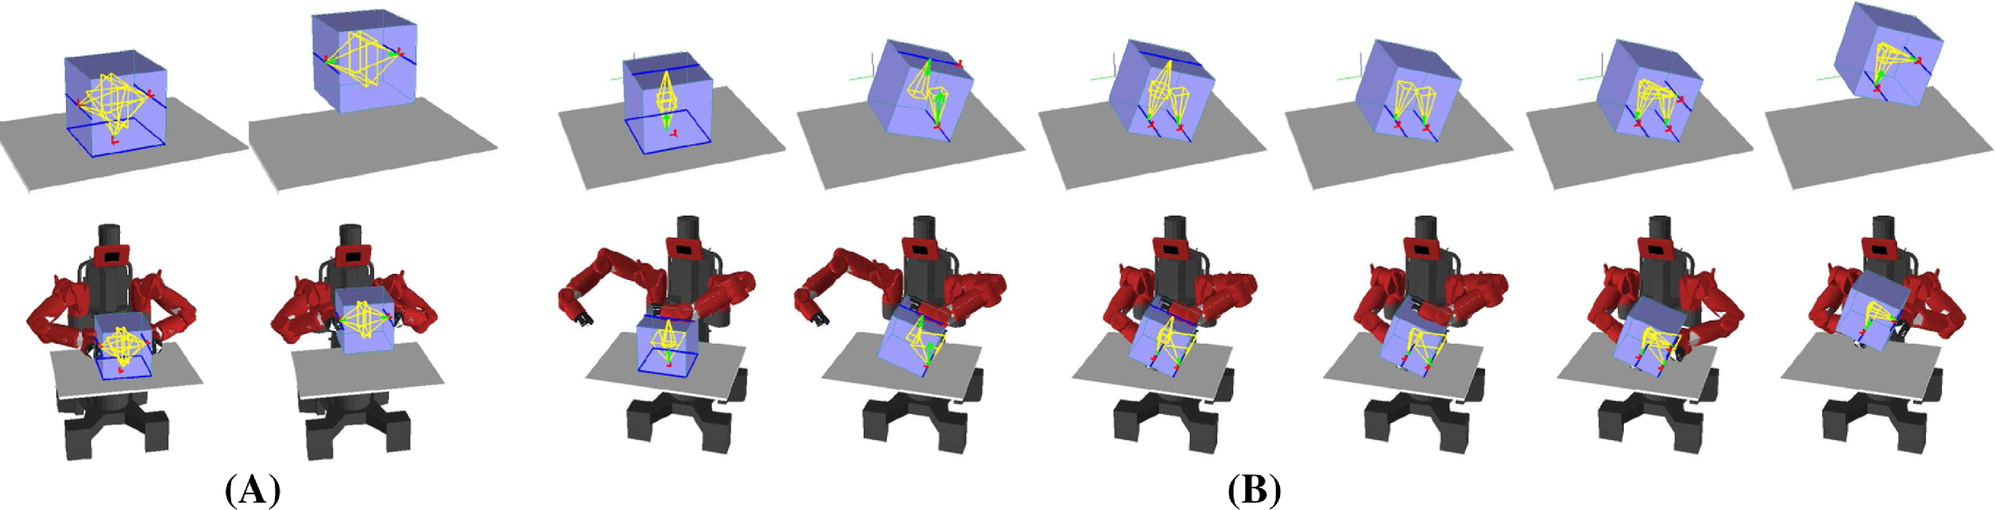
\includegraphics[width=\columnwidth]{figs/baxter_cube_lifting_1}
    \label{figure:baxter_cube_lifting_1}} \\
  \subfloat[]{
    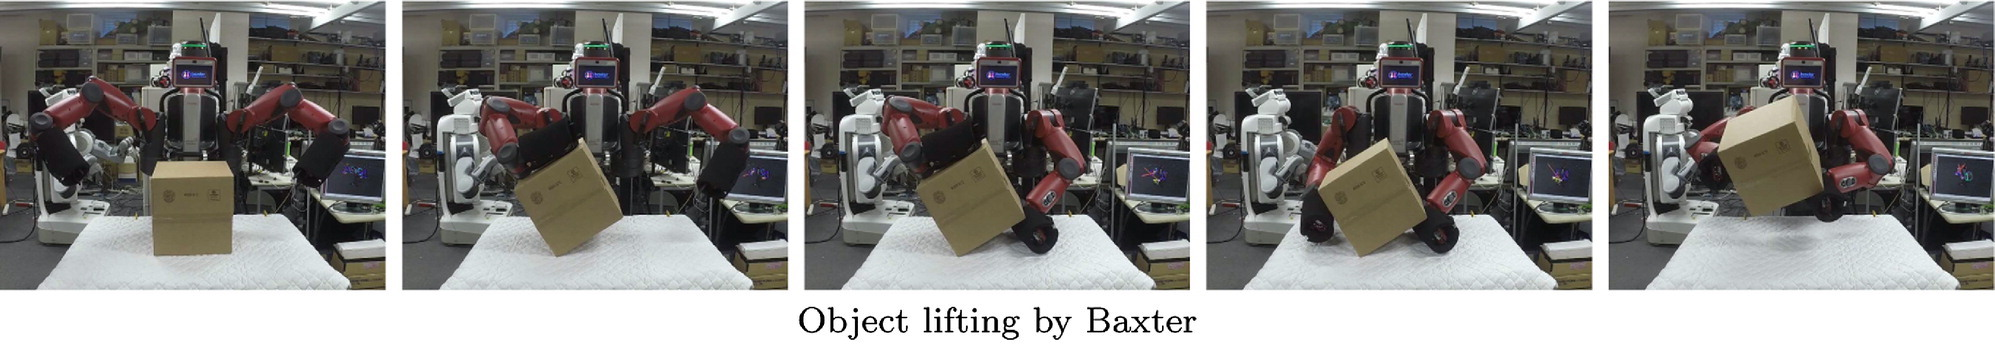
\includegraphics[width=\columnwidth]{figs/baxter_cube_lifting_2}
    \label{figure:baxter_cube_lifting_2}}
  \end{tabular}
  \caption{Cube lifting with 3D Model by a Robot \cite{murooka}}
\end{figure}

このような問題は現状では解決されておらず,物体ピッキング\cite{Ian:DeepGrasp}
以外のより複雑な動作生成においてオンラインで物体モデルを生成し動作計画を行う
ということはロボットの行動実現に関して困難な問題として残っている.
今回,本レポートにおいてこの論文を選択した最も大きな理由はこの問題を解決できる
可能性を持っていると考えるからである.
本節の先に三次元復元に関する画像マッチング技術の応用可能性に関して触れたが,
そこで未知の物体においても二次元画像からの三次元復元が可能であることを述べた.
それは,既知のモデルと新しい物体画像の密なマッチングが取れていれば,
位置物体であるとわかっているがマッチングの無い部分に関しては
補完を行うなどの処理によって未知物体の三次元モデルを
生成可能だと考えられるからである.
論文では同じクラス(猫)ではあるが別の物体(種類の違う猫)に関して
マッチングが成功している例を示しており(\figref{ucn}右),
未知物体への適用可能性が期待できる.
さらにドア開けなどのタスクにおいては,ドアハンドルを認識し,
それを引っ張るなどの動作が必要になり,ハンドルの認識器が必要となる.
通常の物体検出などによるアプローチではドアハンドル専用の認識器が必要となるが,
画像マッチングを用いる場合には,参照している三次元モデルにおけるハンドルの部分と
対応する現実画像の位置に手を伸ばせば良いということになるため未知の物体が含まれていても
対応関係のみを用いてタスクを実現可能である.
これは先の物体認識や物体検出において述べたことと共通している.

\begin{figure}[htbp]
  \centering
  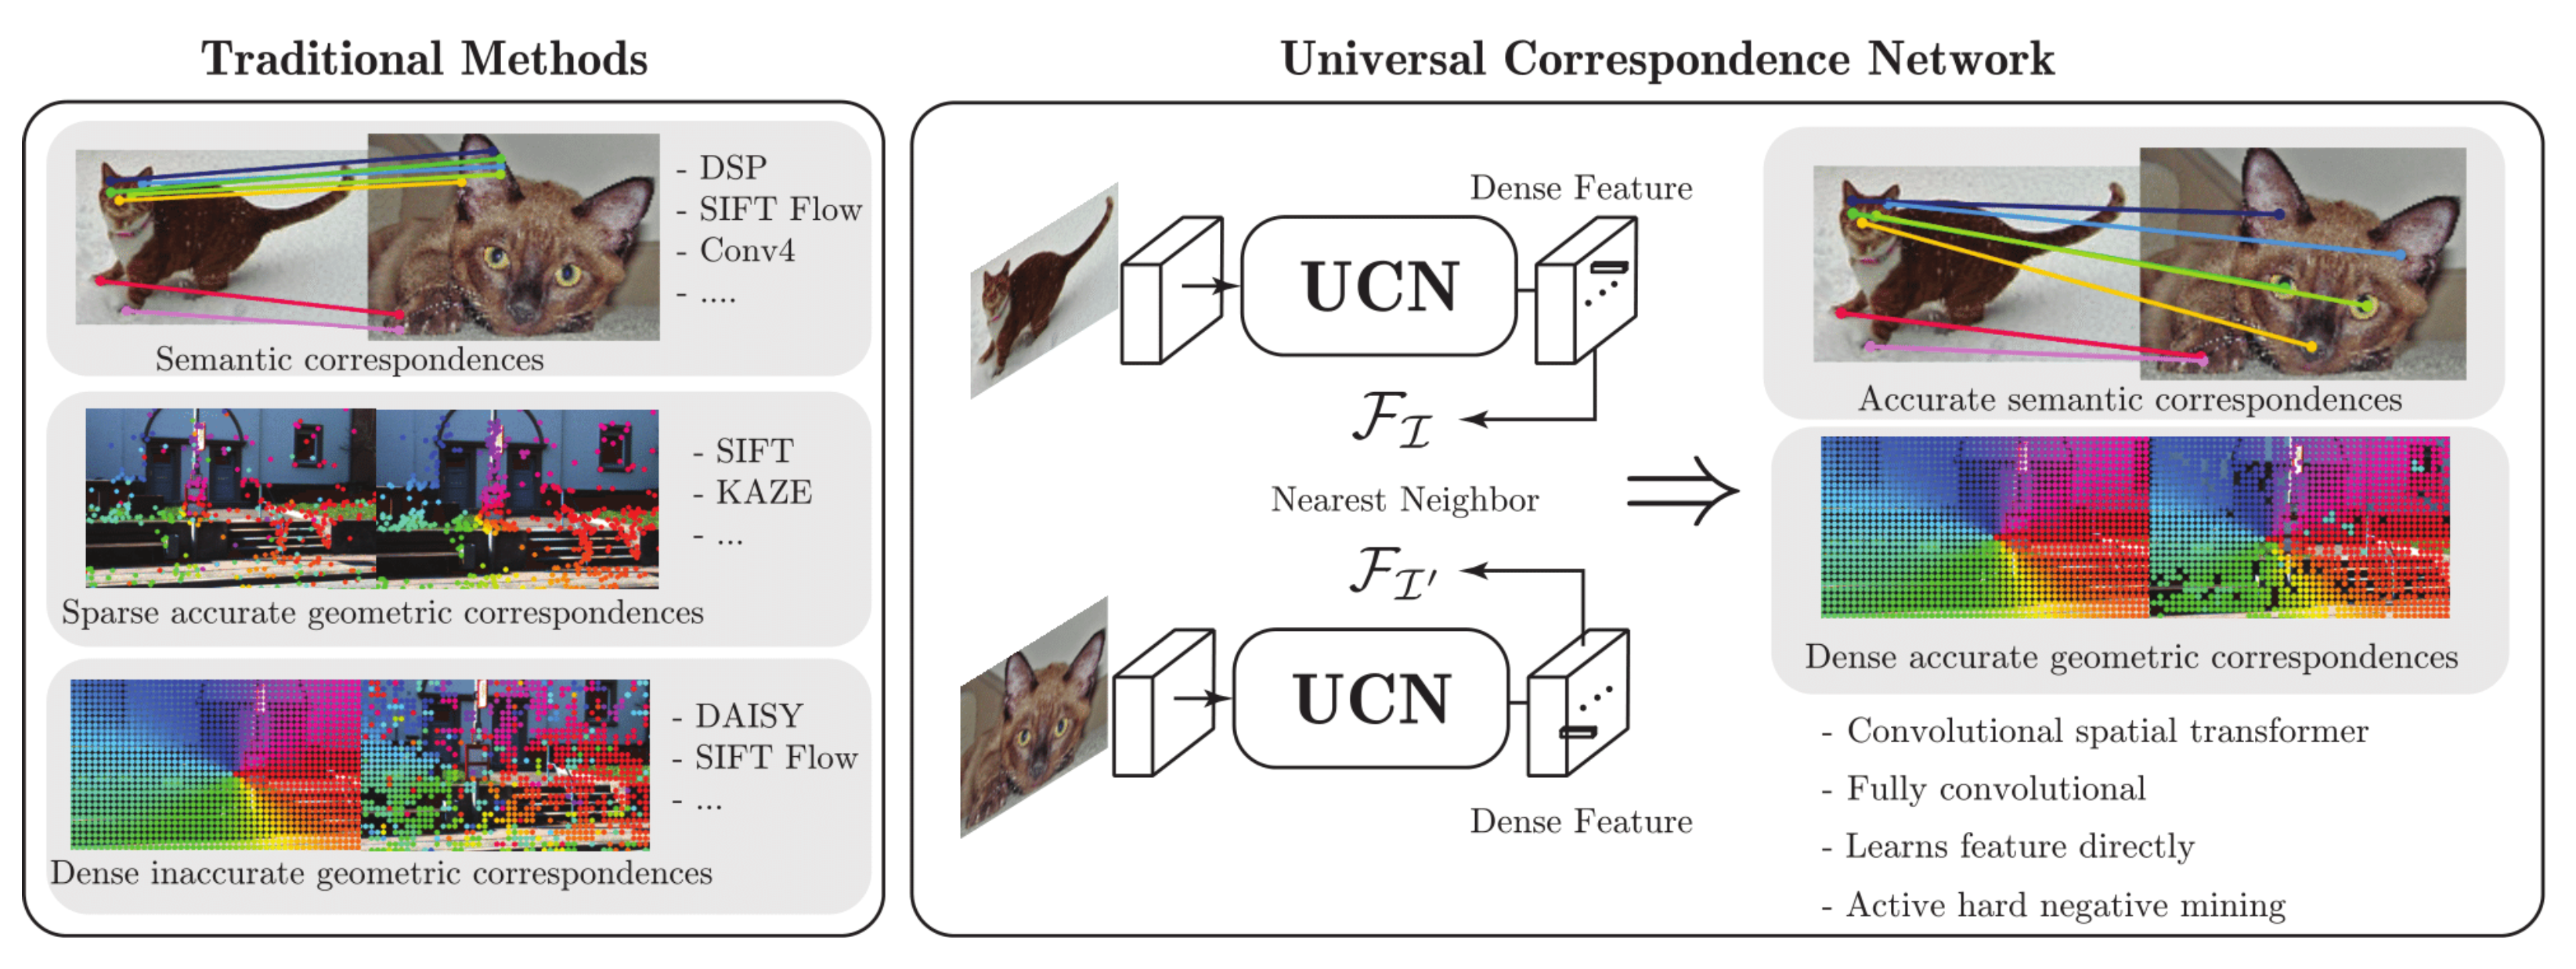
\includegraphics[width=\columnwidth]{figs/ucn}
  \caption{Universal Correspondence Network \cite{choy_nips16}}
  \label{figure:ucn}
\end{figure}

上記に述べたように画像のマッチングは他画像認識タスクへの応用可能性と,
実世界におけるロボットの行動実現に関して非常に有用であり,
高い精度でそれを実現しているこの論文を選択することとした.
